
{\chapter{Conclusions and discussion}

}
\label{ch:Chapter6}

\section{Major findings}
Predicting the dynamics of malignant cells in cancers and deconstructing the molecular basis of resistance and metastasis can be achieved by repeated observation of cell populations with shared genotypes and phenotypes. In this thesis project we have applied this concept to show that cell population dynamics in cancer can be resolved by assigning cells to specific clones, defined by copy number. We repeatedly observe the similar fitness coefficients for the same copy number genotypes, showing deterministic behaviour. The fitness differences between most clones is small, despite large changes in clone prevalence over time.


\subsection{Identification and confirmation of a significant transcriptomic signature under various conditions}

In chapter 3, we set out to assess the impacts of tissue dissociation and data analysis quality control, taking advantage of a recently described protease active at low temperatures (on ice), to contrast the effects of low temperature protease solid tissue dissociation with those of more routinely used collagenase at 37\textdegree C. Identification and confirmation of a significant transcriptomic signature comprising 512 core genes in response to collagenase tissue digestion at 37\textdegree C. Significantly, this signature is highly confounded with known cancer biology, comprising a large number of tumour stress and resistance markers. We demonstrate for the first time that this signature can be mitigated by tissue digestion with a cold protease (active at 6\textdegree C) derived from a Himalayan glacier resident bacterial species.

Predominantly, we FACS sorted lymphoblastoid cells into live, dying, and dead populations (with/without induction of cell death with TNF-alpha) to characterize the efficacy of standard scRNA-seq QC practices on removing dead and dying cells. In doing so, we identify a subset of dead cells which would not be filtered by standard practices. We reported that cells that were FACS sorted as either live, dying, or dead (with/without induction of cell death with TNF-alpha), were present in all three clusters, emphasizing that the although the transcriptomic state and and the surface marker of the cell are correlated but they are not the same. Such concepts are implicative  of ``pseudotime'' in single-cell trajectory analysis, whereby developmentally ordering cells transcriptomically can lead to early or late cells being placed at variable positions along the pseudotime trajectory \cite{campbell2018descriptive, campbell2018uncovering}. 
 Furthermore, we identified a subpopulation of cells (enriched for dying and dead) that showed increased expression of MHC Class I genes, indicative of stress and which may distinguish these cells from otherwise transcriptomically healthy cells. This finding could be pertinent to the studies of immune response in cancer.
 

 Finally, we identified a conserved collagenase-associated transcriptional pattern including induction of stress and heat shock genes, consistent with a transcriptional response identified in a subset of muscle stem cells \cite{van2017single}, and which was minimized when samples were dissociated at cold temperatures with a cold active serine protease. We demonstrate that both digestion time and collagenase contribute to the transcriptomic stress response in single cancer cells. Therefore, the short incubation time necessary for cold protease as well as the relatively stable transcriptome captured by dissociation at cold temperatures suggests this is a potential alternative to collagenase dissociation for scRNA-seq experiments with tumor tissues. We suggest that each tissue and dissociation method should be assessed for dissociation-induced signatures before undertaking large-scale scRNA-seq experiments. 
 
 Transcription of the identified gene set in chapter 3 as a result of sample preparation methods may mask their induction due to other means. For example, \textit{JUN} and \textit{FOS} are associated with cancer drug resistance and metastatic progression \cite{insua2018stress,fan2017ap, ramsdale2015transcription}. Moreover, though less stark as the core collagenase-associated gene set, cell type-specific effects were observed during dissociation and included increased hedgehog and apical surface pathways in breast epithelial cells and reactive oxygen species pathways in cytotoxic T cells and myofibroblasts. Taken together, these findings indicate that all cell types exhibit some level of stress response to dissociation with collagenase, with some cell types exhibiting cell type-specific responses. These stress responses, which may significantly influence the interpretation of scRNA-seq data, are minimized by dissociation at cold temperatures.
 

\subsection{Copy number could be associated with clonal fitness in \textit{Tp53} mutant human breast cancers}
From chapter 4, clonal expansions were observed in \textit{TP53} mutant human breast cancer cells, through serial passaging, single cell sequencing and fitness modeling of four patient derived xenografts. Bulk WGS and DLP+ confirmed all four tumors were p53 mutant (SA609: p.R213X; SA1035: p.C242F; SA532: p.A159P; SA535: frameshift chr17:7578490, \textbf{\autoref{tab:Tp53mutationofPDX}} with bi-allelic and truncal distribution across clones.
We first studied clonal evolution in untreated PDX models, sampled over 927 days for HER2+ SA532, 619 days for TNBC-SA609, 381 days for TNBC-SA1035 and 353 days for TNBC-SA535. DLP+ were generated and sequenced, yielding a median of 1,116 single cell genomes per sample (95,275 total cells). 

All series exhibited progressively higher tumour growth rates over time. In contrast to HER2+SA532, all TNBC PDX models exhibited evidence of clonal diversification associated with copy number alterations and selective coefficients consistent with positive selection over time \textbf{\autoref{fig:landscapefitness}}. 
For TNBC-SA609, Clones E  (1+s= 1.07 $\pm$ 0.02) and H (1+s=1.02 $\pm$ 0.02) had the highest selective coefficients and exhibited growth from undetectable levels to 59 and 32\% respectively by timepoint X10.
In SA535 TNBC, three major clones were observed with clone G characterized by loss of chromosome X exhibiting a clonal expansion from minor prevalence as passage X5 to near dominance at 76\% at passage X9. Similar patterns were observed for the other TNBC cases.  
For TNBC-SA1035, 11 clones were detected with clone E expanding to 69\% at passage X8 from minor prevalence at the initial timepoint. The predicted selective coefficient of clone E was(1+s = 1.06 $\pm$ 0.03) . By contrast, Clones A and K had initial prevalences of 20 and 9\% ,respectively, but were not detectable by the last timepoint. 

Having established quantification of CNA associated subclone fitness, we next asked how clone-specific fitness is influenced under drug treatment. We tested how cisplatin, a standard therapy for primary TNBC, impacted the stability of the fitness landscape of the three independent PDX TNBC series (TNBC-SA609, TNBC-SA535, TNBC-SA1035).

For TNBC-SA609, we implemented a more extensive experimental design to account for potential differences in transplantation from fresh tissues relative to those subjected to a freeze-thaw cycle used in serial propagation between X3 and X4. Three treated lines and Line 2 untreated samples were propagated from an X3 frozen sample, whereas Line 1 untreated samples were propagated from dissociation of a fresh specimen. Technical replicates were also collected for Line 1 and 2.    

In each series, we observed an inversion of the clone fitness landscape \textbf{\autoref{fig:landscapefitness}}, left and right panels), resulting in suppression of clones that dominated in the absence of treatment and emergence of low fitness and/or previously unobserved CNA genotypes. For example, in the treatment branch of TNBC-SA609 Line 2, the growth dynamics over (X3 U; X4 UT; X5 UTT; X6 UTTT; X7 UTTTT) and \textit{fitClone} modeling revealed that resistant clones (A, R)- constituting a branch of the phylogeny derived from clone B,  monotonically increased on treatment. A technical replicate of X7 in Line 2 showed a similar composition and nearly all cells consisted of Clones B and R.  In Line 1, a sibling clone of A, clone R reproducibly swept to fixation on treatment. Notably, after the first treatment cycle, all three lines showed expansion of clone B and its derivative R at timepoint X4 and a contraction of clone H.



\begin{figure}
\centering
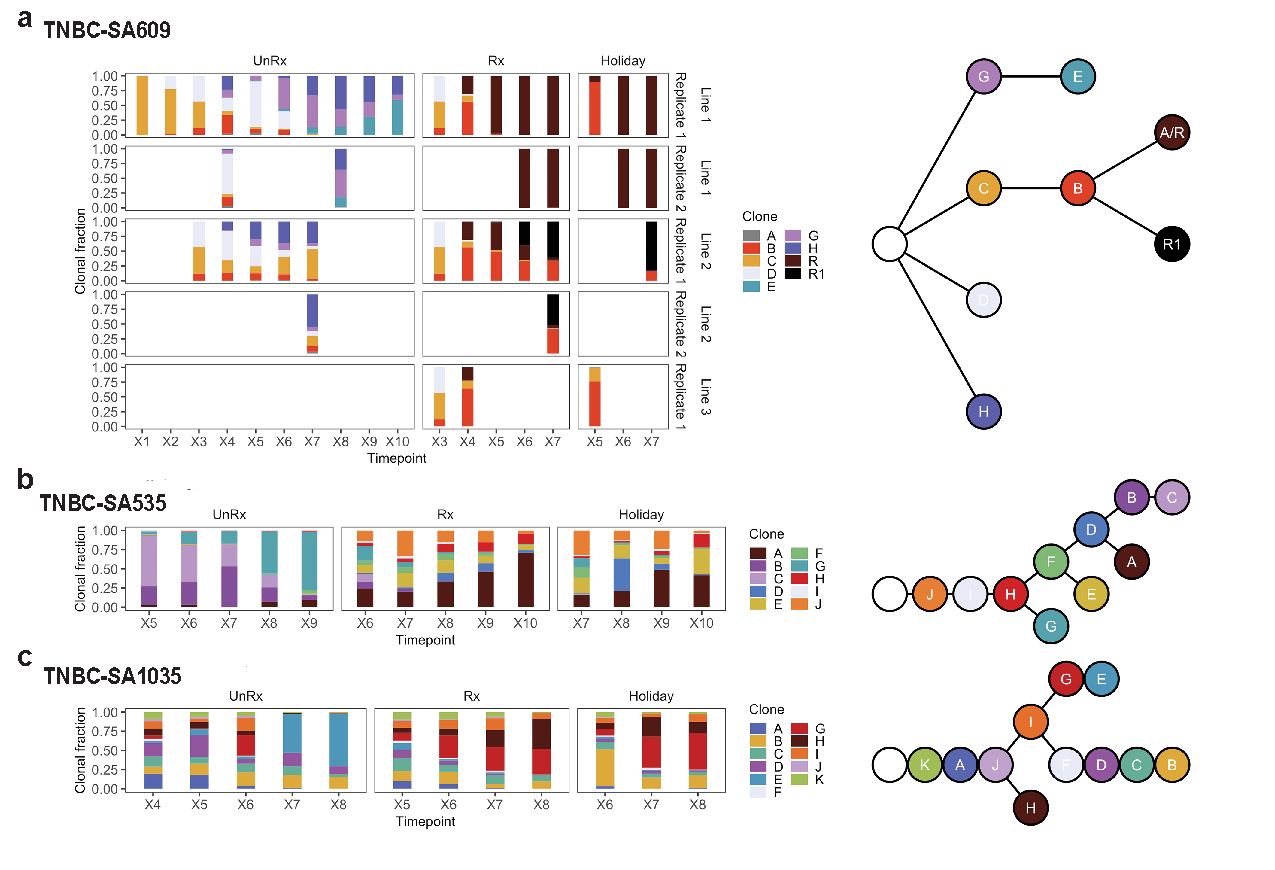
\includegraphics[width=\textwidth]{Figures/All3barplots.pdf}
\caption[Summary of number of genes \textit{in-cis} and \textit{in-trans}]
	{\small
	\textbf{}
	Observed clonal abundances in TNBC-SA609, TNBC-SA535-Rx and TNBC-SA1035-Rx, for each tumor sampled for scWGS. Right vertical axis represents the line. Right panels show clonal phylogenies.
}
    \label{fig:All3barplots}
    \end{figure}

Notably, the high fitness clones H, G, D from the untreated series exhibited low fitness coefficients in the treatment series and were no longer detected \textbf{\autoref{fig:landscapefitness}}. This was evident in the relative fitness ranking \textbf{\autoref{fig:landscapefitness} d}, clone bipartite fitness rank) and absolute fitness values (reffig{fig:landscape} d, probability of positive selection). Conversely, Clones A, B,  and C, comprising a low fitness phylogenetic superclade, distinct from high fitness clone H in the untreated series, were the precursors to the resistant clone R \textbf{\autoref{fig:landscapefitness}}, \textbf{\autoref{fig:All3barplots}}. 

In the TNBC-SA535 and TNBC-SA1035 treatment series, similar patterns of low fitness clones in the untreated series expanding on treatment (clone A, in TNBC-SA535; clones G, H, in TNBC-SA1035), with the fittest clones under no treatment (e.g. TNBC-SA535 clone G; TNBC-SA1035 clone E) decreasing to near zero prevalence. The majority of the other clones were also impacted by treatment in all three series. For example, in SA535, the relative fitness rank of Clone G fell from first to sixth and clone B fell from third to tenth.  Clone H increased from sixth to second and Clone J from seventh to third.  

In SA1035, Clone E fell from first to seventh and clone A fell from third to eighth. Clone G increased from tenth to second.  The impact across the whole fitness landscape was reflected in the probability of positive selection distributions.  These distributions were statistically significantly increased in the treatment series  (\textbf{\autoref{fig:landscapefitness}} d), indicating that fewer clones were under neutral selection as a function of cisplatin, and that the fitness landscape exhibited a wider variance between clones.

For example, in the treatment branch of TNBC-SA609 replicate treated, Line 2, the growth dynamics over (X3 U; X4 UT; X5 UTT; X6 UTTT; X7 UTTTT) and \texttt{fitClone} modeling revealed that a new ``Clone R1'', constituting a branch of the phylogeny derived from clone B, monotonically increased on treatment.  A technical replicate of X7 in Line 2 showed a similar composition, nearly all cells consisted of Clones B and R1.  In Line 1 a sibling clone of R1, clone R reproducibly swept to fixation on treatment.  Notably, after the first treatment cycle, all three lines showed expansion of clone B and its derivative R at timepoint X4 and a contraction of clone H.

Moreover, the heat maps of TNBC-SA609 and TNBC-SA535 PDX \textbf{(\autoref{fig:mediangenotypes}}) exhibited more complex heterogeneity at copy number space along with structural genomic rearrangements as compared to TNBC-SA1035 PDX.


\subsection{Clone specific genotypes drives clone-specific gene expression programs}

After establishing the fitness of genomic clones in the presence or absence of chemotherapies in chapter 4, we next sought to uncover the basis of how copy number variation alters gene expression in complex cell mixtures. In parallel, we sequenced single-cell RNA from independent cell populations and mapped for genome-transcriptome association. 
We revealed that gene expression states can be assigned to cancer clones using single-cell RNA and DNA sequencing independently sampled from a heterogeneous cell populations. We also demonstrated that single cell RNAseq clusters exhibited comparably monomorphic pattern of global expression over time which could be tracked with clonal assignments.

%----------------------------------------------------------

 \begin{table}[htbp]
   \centering
   \caption{Number of genes in DE* of resistant versus sensitive clones and their regulation status in all TNBC PDX series}
     \begin{tabular}{|l|l|l|}
     \hline
     \multicolumn{1}{|l|}{\textbf{No. of genes**}} & \multicolumn{1}{|l|}{\textbf{Percent genes (\%)}} & \textbf{Gene regulation} \\
     \hline
     \multicolumn{1}{|l|}{\textbf{SA609-TNBC}} &   &  \\
     438 & 12.9 & In\_cis\_Decrease\_DownRegulated \\
     76 & 2.2 & In\_cis\_Decrease\_UpRegulated \\
     214 & 6.3 & In\_cis\_Increase\_DownRegulated \\
     926 & 27.3 & In\_cis\_Increase\_UpRegulated \\
     966 & 28.4 & In\_trans\_DownRegulated \\
     778 & 22.9 & In\_trans\_UpRegulated \\
     \multicolumn{1}{|l|}{\textbf{SA1035-TNBC}} &   &  \\
     93 & 2.6 & In\_cis\_Decrease\_DownRegulated \\
     18 & 0.5 & In\_cis\_Decrease\_UpRegulated \\
     19 & 0.5 & In\_cis\_Increase\_DownRegulated \\
     116 & 3.3 & In\_cis\_Increase\_UpRegulated \\
     1661 & 47.2 & In\_trans\_DownRegulated \\
     1612 & 45.8 & In\_trans\_UpRegulated \\
     \multicolumn{1}{|l|}{\textbf{SA535-TNBC-cisplatin}} &   &  \\
     473 & 9.8 & In\_cis\_Decrease\_DownRegulated \\
     271 & 5.6 & In\_cis\_Decrease\_UpRegulated \\
     43 & 0.9 & In\_cis\_Increase\_DownRegulated \\
     253 & 5.2 & In\_cis\_Increase\_UpRegulated \\
     1068 & 22.1 & In\_trans\_DownRegulated \\
     2716 & 56.3 & In\_trans\_UpRegulated \\
     \multicolumn{1}{|l|}{\textbf{SA535-TNBC-CX-5461}} &   &  \\
     697 & 21.5 & In\_cis\_Decrease\_DownRegulated \\
     91 & 2.8 & In\_cis\_Decrease\_UpRegulated \\
     45 & 1.4 & In\_cis\_Increase\_DownRegulated \\
     345 & 10.6 & In\_cis\_Increase\_UpRegulated \\
     924 & 28.5 & In\_trans\_DownRegulated \\
     1145 & 35.3 & In\_trans\_UpRegulated \\
     \hline
     \end{tabular}%
     
   \label{tab:NumberofDEgenesandstatus}%
   
   \small\textbf{(*Differential expression, ** (FDR$<$0.01, p$<$0.05))}.
 \end{table}%

%----------------------------------------------------------

Importantly, we were able to dissect the regulation status of  differentially expressed genes between genomically defined resistant and sensitive clones in all TNBC PDX series. For example, pairwise comparisons of clone-specific differential gene expression in \textbf{SA609} , between resistant clone R and sensitive clone H (FDR$<$0.01, p$<$0.05), identified 926 genes having clone specific copy number increase in expression \textit{(incis\_IU)}, whereas, 438 genes were downregulated with decrease in copy number \textit{(incis\_DD)}. Whereas, 966 genes were downregulated and 778 were upregulated  independent of change in copy number \textit{in trans} \textbf{(\autoref{fig:Volcanotrackplots2.pdf} a, left)}, Summary of all 4 PDX series \textbf{\autoref{tab:NumberofDEgenesandstatus}}. The Manhattan plot confirming the increase and decrease in copy number between clones at that genomic position and its respective change in gene expression \textbf{(\autoref{fig:Volcanotrackplots2.pdf} a, right)}.

In high fitness clones (resistant) with amplifications as distinguishing features, we noted accompanying \textit{in cis} clone-specific differential gene expressions, for example, in SA609-TNBC, \textit{CRABP1} in resistant clone of SA609 TNBC PDX (clone R with copies of Chr15q) and  \textit{TCF4} in clone R with 3 copies of Chr20q). Summary of top 20 clone specific upregulated genes and their change in copy number are in \textbf{Chapter 5}.

Together these data indicate that clonal genotypes driving high fitness trajectories are accompanied by changes in gene expression at both chromosomal and focal level copy number alterations with variable individual gene regulation status.


\section{Limitations and future directions}

IN chapter 3, our novel and single cell RNA seq analysis data provided a comprehensive set of information regarding tissue handling and its effects on sequencing analysis and biological interpretation. Though cell type-specific gene expression effects in response to digestion method were evident, these findings indicate that all cell types exhibit some level of stress response to dissociation with collagenase, with some cell types exhibiting cell type-specific responses. 
However, in large scale drug studies where stress is also induced by chemotherapies and we are interested in studying various relationships of pathways and its downstream effectors, we need to be careful in making choices of digestion enzymes and conditions. 

Another limitation using cold active protease enzyme is that, we didn't compared simultaneously the \ac{DLP+} libraries alongside single cell RNA sequencing at different temperatures. In future, we plan to directly investigate the difference of single cell whole genome sequencing, by comparing digestion at 6\textdegree C and at 37\textdegree C. In addition, while performing our experiments for chapter 3, we noticed that digestion at cold temperature tend to lose more number of cells as compared to digestion at 37\textdegree C. This factor play an important role where we need to make multiple measurements form the same tumor. Moreover, the type of tissue, its consistency and its exposure to either chemotherapy or environmental and genetic perturbations should also be considered as a factor. The choice of digestion enzyme and temperature should be optimized accordingly with before conducting any large scale study.

In chapter 4, we demonstrated a timeseries model of cisplatin resistance in TNBC PDX, which is a standard care and first line of systemic treatment given in most of the cancers. We were intended to explore the underlying clonal dynamics that undergo a change with and without any perturbations to the tumor environment that ultimately lead to tumor resistance. We recognize that establishing causal relationships based on copy number clustering into clones is very difficult and requires more controlled experiments and larger sample sizes. However, exploring the potential correlates of differential fitness may aid in designing follow up experiments. In our timeseries experiments, two out of four PDX series exhibited directional dynamics over either serial passaging or drug intervention. The untreated dynamics were confirmed by two different sets of mixture experiments. In future, more mixture experiments for the timeseries that undergo neutral dynamics over time will explain the tumor biology explicitly. 

Furthermore, in the context of pharmacological intervention, we acknowledge that the drug exposure started from early time points that derives the competition among the clones and infer the fitness of certain clones. It would be very interesting and comparable to conduct experiments where we take later passages of the time series PDXs and start introducing the chemotherapy in the same way. Clonal competitions and fitness in that environment will become obvious.

Pseudobulk, that is merging of single cells to create more sequencing depth for SNV detection is not explained in detail in chapter 4. All the data is being processed and under investigations for SNVs, detailed mutational analysis and integration of allelic imbalance information caused by clone-specific \ac{LOH} events. Follow up replication experiments sequenced at higher depth may be required to rule out the existence of driving mutations. 


In chapter 5, laveraging the newly developed clonealign statistical model,the focus has been on linking transcriptional measurements to genomically defined clones assuming only a copy-number dosage effect on transcript abundance. While the clonealign model allows for integration of allelic imbalance information caused by clone-specific \ac{LOH} events, the sparse expression of germline heterozygous variants detected by the 10X chromium 3' assay demonstrated here makes such information uninformative. However, full-transcript-length single-cell RNA sequencing technologies such as Smart-seq2 \cite{picelli2014full} would allow for further refinement of clonal assignment and represent the appropriate use-case of clonealign’s incorporation of allelic imbalance information.


Furthermore, we explored single cell expression in reference to resistant and sensitive clones defined in the previous chapter. Notable, we indentify many new pathways and genes playing role in our TNBC time series, that are not well studied in context of breast cancer. We have the data of genes that are regulated \textit{in cis} or \textit{in trans}. If there is a loss of copy number that is leading to resistant phenotype, not much could be done, but if the gene is upregulated \textit{in trans}, independent of change in copy number, it could act as a tumor biomarker and gene editing through CRISPRi \cite{larson2013crispr}, for example could be a potential follow up experiment.
Other future experiments would be to use CRISPR/cas9 \cite{doudna2014new} technology for biomarker validations. We have enlisted various combinations of genes, where some are commonly showed up in all treated time series while, some are more specific to certain PDXs. 

Another supporting biological methodology involves epigenetic changes, that may influence the fitness of clones and interrogating the system via orthogonal data types such as chromatin accessibility and/or DNA methylation assays. This is important coupling with single cell RNA expression in context of measuring to gene promoters hypermethylation of tumor suppressor genes  or hypomethylation of oncogenes.








 
 
 
 
 
 
 Single cell RNA seq analysis data can help in a better comprehension of some widespread and more specific biological mechanisms involved in breast cancer progression.that could be further validated pertaining to drug resistance in triple negative through modern techniques, such as, CRISPR/Cas9.

Genetic alterations and the contextual signaling by the microenvironment give rise to an intricate network of pathological mechanisms and molecular pathways


Individual tumors and cancer cells exhibit substantial molecular diversity.

Single cell RNA seq analysis data can help in a better comprehension of some widespread and more specific biological mechanisms involved in breast cancer progression.